% Póster científico · Expo Ingenierías (versión 1, diseño propio)
% Compilar con LuaLaTeX:  lualatex poster1.tex   (gráficas: Rscript figuras_poster.R)
\documentclass{article}
\usepackage[paperwidth=90cm,paperheight=120cm,margin=0cm]{geometry}
\usepackage{fontspec}
\usepackage[spanish,es-noshorthands]{babel}
\usepackage{xcolor,graphicx,tikz,enumitem,tabularray,qrcode}
\usepackage[most]{tcolorbox}
\usetikzlibrary{positioning,arrows.meta,calc,shapes.symbols,shadows}
\pagestyle{empty}
\setlength{\parindent}{0pt}
\setlength{\parskip}{0pt}

% ---------- letra: Source Sans 3 (texto) y Source Serif 4 (títulos)
\setmainfont{SourceSans3}[Extension=.otf, UprightFont=*-Regular, BoldFont=*-Bold, ItalicFont=*-RegularIt, BoldItalicFont=*-BoldIt, FontFace={sb}{n}{*-Semibold}, FontFace={k}{n}{*-Black}]
\newfontfamily\serif{SourceSerif4}[Extension=.otf, UprightFont=*-Regular, BoldFont=*-Bold, ItalicFont=*-RegularIt, FontFace={sb}{n}{*-Semibold}, FontFace={k}{n}{*-Black}]
\newcommand\sbf{\fontseries{sb}\selectfont}
\newcommand\blk{\fontseries{k}\selectfont}

% ---------- colores (los mismos de las gráficas)
\definecolor{tinta}{HTML}{1D2440}
\definecolor{gris}{HTML}{6B6F80}
\definecolor{papel}{HTML}{FBF8F2}
\definecolor{crema}{HTML}{F3EEE3}
\definecolor{linea}{HTML}{E2DCCD}
\definecolor{hogar}{HTML}{C8553D}
\definecolor{escuela}{HTML}{2E6FA7}
\definecolor{bajo}{HTML}{C9C6DD}
\definecolor{medio}{HTML}{8C86B8}
\definecolor{alto}{HTML}{3C3570}
\definecolor{oro}{HTML}{E9B44C}
\pagecolor{papel}
\color{tinta}

% ---------- tamaños
\newcommand\cuerpo{\fontsize{24}{31.5}\selectfont}
\newcommand\chico{\fontsize{20.5}{26}\selectfont}
\newcommand\mini{\fontsize{17.5}{22}\selectfont}
\newlength\colw \setlength\colw{26.4cm}
\newlength\gut \setlength\gut{2.4cm}

% título de sección: número en círculo, título en serif y una línea
\newcommand\seccion[2]{%
  \par\vspace{0.9cm}%
  \begin{tikzpicture}[baseline=(t.base)]
    \node[circle, fill=tinta, text=papel, minimum size=2.1cm, inner sep=0, font=\serif\bfseries\fontsize{46}{46}\selectfont] (n) {#1};
    \node[right=0.7cm of n, anchor=west, font=\serif\bfseries\fontsize{54}{60}\selectfont, text=tinta] (t) {#2};
  \end{tikzpicture}\par\vspace{0.35cm}%
  {\color{linea}\rule{\linewidth}{4pt}}\par\vspace{0.55cm}}
\newcommand\sub[1]{\par\vspace{0.7cm}{\serif\sbf\fontsize{36}{42}\selectfont\color{alto}#1}\par\vspace{0.4cm}}
\newcommand\fig[2]{\par\vspace{0.5cm}\includegraphics[width=\linewidth]{figs/#1}\par\vspace{0.25cm}{\chico\color{gris}#2}\par}
\newtcolorbox{prueba}[1][]{enhanced, colback=white, colframe=white, boxrule=0pt, arc=10pt,
  borderline west={10pt}{0pt}{#1}, left=30pt, right=26pt, top=20pt, bottom=20pt, before skip=0.7cm, after skip=0.3cm,
  fontupper=\chico, drop fuzzy shadow={black!25}}
\setlist[itemize]{leftmargin=1.3cm, label={\color{oro}\raisebox{0.12em}{\scalebox{1.4}{$\bullet$}}}, itemsep=0.2cm, topsep=0.2cm, parsep=0pt}
\newcommand\hz{H\textsubscript{0}}
\newcommand\ha{H\textsubscript{1}}

\begin{document}
\cuerpo
% =================================================================== ENCABEZADO
\begin{tikzpicture}[remember picture, overlay]
  \fill[tinta] (current page.north west) rectangle ([yshift=-18.6cm]current page.north east);
  % lomos de libros sobre el borde inferior del encabezado
  \foreach \x/\h/\c in {0/1.5/hogar, 1.4/2.0/oro, 2.5/1.3/escuela, 3.7/1.8/medio, 4.9/1.4/hogar, 6.0/2.1/bajo, 7.3/1.6/oro, 8.4/1.9/escuela,
                        77.0/1.8/escuela, 78.2/1.4/oro, 79.3/2.1/hogar, 80.7/1.6/medio, 81.9/1.9/bajo, 83.2/1.3/escuela, 84.3/1.8/oro, 85.6/1.5/hogar, 86.8/2.0/medio, 88.1/1.6/bajo}
    \fill[\c] ([xshift=\x cm, yshift=-18.6cm]current page.north west) rectangle ++(1.05, \h);
  \node[anchor=north west, fill=white, rounded corners=14pt, inner sep=22pt] at ([xshift=3cm, yshift=-1.3cm]current page.north west) {
\includegraphics[height=2.1cm]{img/tec_logo.png}};
  \node[anchor=north east, align=right, text=papel!85!tinta, font=\sbf\fontsize{26}{34}\selectfont] at ([xshift=-3cm, yshift=-1.5cm]current page.north east)
    {Expo Ingenierías · 28.ª edición\\[2pt] \fontseries{m}\selectfont Investigación y desarrollo de propuestas de mejora\\ MA1001B Modelación estadística para la toma de decisiones};
  \node[anchor=north, text width=78cm, align=center, text=white, font=\serif\bfseries\fontsize{84}{94}\selectfont] (titulo) at ([yshift=-5.3cm]current page.north)
    {Desigualdad en el acceso a la lectura en la infancia\\ y su impacto en los hábitos de lectura en la vida adulta};
  \node[anchor=north, below=0.45cm of titulo, text=oro, font=\serif\itshape\fontsize{40}{46}\selectfont] (subt) {Análisis estadístico del Módulo sobre Lectura (MOLEC) del INEGI, 2019–2024};
  \node[anchor=north, below=0.55cm of subt, text width=80cm, align=center, text=white, font=\sbf\fontsize{30}{40}\selectfont] (aut)
    {Fernando Isaac Martínez García \enspace·\enspace Mateo Rodolfo Flores Torres \enspace·\enspace Eliel Silva Morales \enspace·\enspace César Julián Leal Salazar};
  \node[anchor=north, below=0.35cm of aut, text=papel!75!tinta, font=\fontsize{24}{32}\selectfont] (tut)
    {Tutoras: Dra. Blanca Rosa Ruiz Hernández y Dra. María Guadalupe Tobías Lara \enspace·\enspace Tecnológico de Monterrey, Campus Monterrey};
\end{tikzpicture}
\vspace*{18.6cm}

% =================================================================== FRANJA DEL HALLAZGO
\begin{tikzpicture}
  \fill[crema] (0,0) rectangle (90,-10.6);
  \node[anchor=north west, text width=27cm, font=\serif\bfseries\fontsize{37}{45}\selectfont, text=tinta] at (3,-1.2)
    {Con acceso alto a la lectura en el hogar durante la infancia, la proporción de adultos lectores es \textcolor{hogar}{aproximadamente el doble} que con acceso bajo.};
  \node[anchor=north west, text width=27cm, font=\mini, text=gris] at (3,-8.5) {Asociación, no causalidad · 96\,\% de confianza · α = 0.04 · 11,685 adultos alfabetos de 32 áreas urbanas};
  % cuatro cifras
  \foreach \i/\num/\col/\txt in {
      0/41.7\,\%/tinta/{leyó al menos un libro\\en los últimos 12 meses},
      1/{28.1\,\% \textcolor{gris}{\fontseries{m}\selectfont vs} 59.7\,\%}/alto/{lectores con acceso bajo\\vs alto en el hogar},
      2/{46.4\,\% \textcolor{gris}{\fontseries{m}\selectfont vs} 27.0\,\%}/hogar/{lectores con estímulos solo en\\el hogar vs solo en la escuela},
      3/{+0.78}/escuela/{libros al año (acceso alto − bajo);\\IC 96\,\%: 0.43 a 1.13}} {
    \node[anchor=north west, fill=white, rounded corners=16pt, minimum width=13.0cm, minimum height=8.2cm, drop shadow={opacity=0.12}] (c\i) at ({32.5+\i*13.75},-1.2) {};
    \node[anchor=north, font=\serif\bfseries\fontsize{44}{52}\selectfont, text=\col, text width=12.2cm, align=center] at ($(c\i.north)+(0,-1.1)$) {\num};
    \node[anchor=north, font=\fontsize{21}{27}\selectfont, text=tinta, text width=12cm, align=center] at ($(c\i.north)+(0,-3.9)$) {\txt};
  }
\end{tikzpicture}

% =================================================================== TRES COLUMNAS
\hspace*{3cm}%
% ------------------------------------------------------------ columna 1
\begin{minipage}[t]{\colw}
\seccion{1}{El problema}
En México solo cerca de cuatro de cada diez adultos alfabetos leen libros: en la muestra analítica, \textbf{41.7\,\%} leyó al menos uno en el último año, y quienes leen leyeron en promedio \textbf{3.5} libros (12.6 en Estados Unidos; Gallup, 2022). Entre 2015 y 2024, la población alfabeta que lee algún material bajó de 84.2\,\% a 69.6\,\% (INEGI, 2024).\par\vspace{0.5cm}
El hábito lector adulto depende de las oportunidades tempranas de contacto con libros y con adultos lectores. Los libros en casa transmiten \textbf{capital cultural} (Bourdieu, 1986); crecer con muchos libros se asocia con 3 años más de escolaridad en 27 países (Evans et al., 2010), y la lectura conjunta, con mejores resultados de lectura (Bus et al., 1995).

\seccion{2}{Pregunta y objetivos}
\begin{tcolorbox}[enhanced, colback=tinta, colframe=tinta, arc=14pt, left=30pt, right=30pt, top=24pt, bottom=24pt, fontupper=\color{white}\fontsize{28}{37}\selectfont]
{\serif\itshape ¿Cómo se relaciona la desigualdad en el acceso a la lectura durante la infancia con los hábitos de lectura de libros en la edad adulta?}\par\vspace{0.5cm}
{\color{oro}\sbf a)} con la decisión de leer o no leer libros;\par
{\color{oro}\sbf b)} con la cantidad de libros leídos.
\end{tcolorbox}
\vspace{0.3cm}
\begin{itemize}
  \item Construir dos índices de acceso: hogar y escuela.
  \item Evaluar si ambos accesos son independientes.
  \item Comparar estímulos solo en casa vs solo en la escuela.
  \item Comparar la media de libros leídos según el acceso.
\end{itemize}

\seccion{3}{Datos y método}
\begin{center}
\begin{tikzpicture}[font=\chico, every node/.style={align=center},
    caja/.style={draw=linea, line width=3pt, fill=white, rounded corners=12pt, inner sep=16pt},
    flecha/.style={-{Latex[length=0.7cm,width=0.6cm]}, line width=4pt, color=gris!70}]
  \node[caja, text width=10.4cm] (b) {\sbf 6 levantamientos del MOLEC\\ 2019–2024 · 11,966 personas};
  \node[caja, right=3.2cm of b, text width=8.6cm, fill=tinta, draw=tinta, text=white] (m) {\sbf Muestra analítica\\ \fontsize{40}{46}\selectfont\serif\bfseries 11,685 \\ \chico adultos alfabetos};
  \draw[flecha] (b) -- node[above, font=\mini, text=gris] {−281 que} node[below, font=\mini, text=gris] {no leen} (m);
  \node[caja, anchor=north west, at={($(b.west |- m.south)+(0,-1.6)$)}, text width=10.6cm, draw=hogar, align=left] (h)
    {{\sbf\color{hogar} Índice del hogar} (0 a 4)\\[4pt]\mini La llevaban a bibliotecas o librerías · veía leer a sus padres · le leían · había libros en casa};
  \node[caja, anchor=north east, at={($(m.south east)+(0,-1.6)$)}, text width=10.6cm, draw=escuela, align=left] (e)
    {{\sbf\color{escuela} Índice de la primaria} (0 a 4)\\[4pt]\mini Le pedían leer otros libros · comentar lo leído · la motivaban a leer · la animaban a ir a bibliotecas};
  \draw[flecha] (m.south) -- ++(0,-0.7) -| (h.north);
  \draw[flecha] (m.south) -- ++(0,-0.7) -| (e.north);
  \node[below=0.7cm of $(h.south)!0.5!(e.south)$, font=\chico] (n) {Niveles de acceso: \;
    \tikz[baseline=-0.6ex]\node[circle, fill=bajo, minimum size=0.8cm]{}; bajo (0–1) \;
    \tikz[baseline=-0.6ex]\node[circle, fill=medio, minimum size=0.8cm]{}; medio (2) \;
    \tikz[baseline=-0.6ex]\node[circle, fill=alto, minimum size=0.8cm]{}; alto (3–4)};
\end{tikzpicture}
\end{center}
\vspace{0.2cm}
{\chico Ocho preguntas de la infancia (p34a–d y p36a–d) se combinaron en dos índices; quien respondió «No recuerda» quedó como dato faltante. Los porcentajes son de la muestra (sin factor de expansión). Análisis en R con \textbf{α = 0.04} (96\,\% de confianza).}
\par\vspace{0.4cm}
{\mini
\begin{tblr}{colspec={X[1.15,l] X[0.32,c] X[1.7,l]}, width=\linewidth, row{1}={font=\sbf, bg=crema}, rowsep=7pt, colsep=10pt, hline{1,Z}={2pt,tinta}, hline{2}={1pt,tinta}, hline{3-Y}={0.6pt,linea}}
Técnica & Preg. & Supuesto y verificación \\
IC y prueba z de proporciones & a) & n·p ≥ 5 y n·(1 − p) ≥ 5 en cada grupo (mínimo 232) \\
Ji-cuadrada de independencia & a) & Frecuencias esperadas ≥ 5 (mínima 184.8) \\
IC y prueba t de Welch & b) & Libros no normales (Shapiro-Wilk, p < 0.001); más de 1,400 por grupo: TLC. Varianzas distintas (F = 1.21) \\
\end{tblr}}
\end{minipage}%
\hspace{\gut}%
% ------------------------------------------------------------ columna 2
\begin{minipage}[t]{\colw}
\seccion{4}{¿Leer o no leer?}
{\sbf Descriptivo.} El porcentaje de lectores sube con cada estímulo recibido en la infancia, más en el hogar que en la escuela.
\fig{f1_estimulos.pdf}{Porcentaje de personas que leyó al menos un libro, según el número de estímulos en el hogar y en la primaria.}

\sub{Intervalos de confianza al 96\,\%}
Con 96\,\% de confianza, lee libros entre \textbf{26.8\,\% y 29.3\,\%} de quienes tuvieron acceso bajo en el hogar, contra \textbf{58.1\,\% y 61.3\,\%} de quienes tuvieron acceso alto. \textbf{Los intervalos no se traslapan.}
\fig{f2_ic_niveles.pdf}{Proporción de lectores e IC al 96\,\% por nivel de acceso. Pruebas z entre niveles: se rechaza \hz{} en las 6 comparaciones (z de 3.37 a 30.50; frontera ±2.054).}

\sub{Con la misma escolaridad}
La escolaridad, indicador indirecto del nivel socioeconómico, también se asocia con leer. Aun así, dentro de cada nivel escolar, el acceso alto se asocia con \textbf{19 a 24 puntos más} de lectores.
\fig{f3_escolaridad.pdf}{Porcentaje de lectores por escolaridad y nivel de acceso en el hogar.}
\end{minipage}%
\hspace{\gut}%
% ------------------------------------------------------------ columna 3
\begin{minipage}[t]{\colw}
\seccion{5}{¿Hogar o escuela?}
\begin{minipage}[t]{12.4cm}\vspace{0pt}
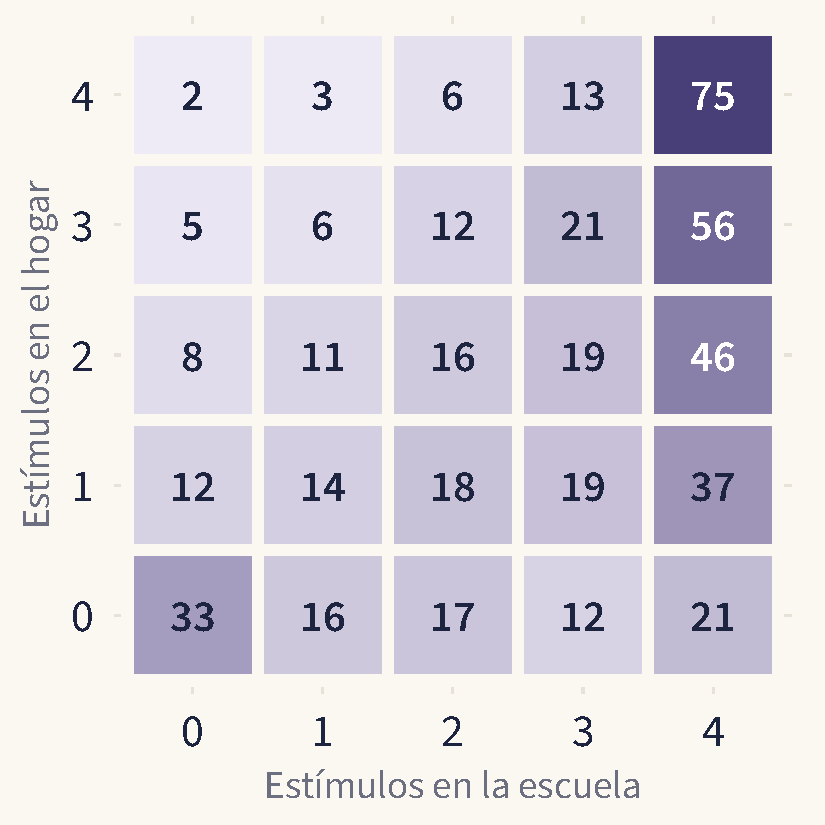
\includegraphics[width=\linewidth]{figs/f4_contingencia.pdf}
\end{minipage}\hfill
\begin{minipage}[t]{13.4cm}\vspace{0.3cm}
{\chico Porcentaje por renglón: de quienes recibieron 4 estímulos en casa, 75\,\% también recibió 4 en la escuela; de quienes no recibieron ninguno, solo 21\,\%.}
\begin{prueba}[alto]
{\sbf Prueba ji-cuadrada}\\ \hz: los dos índices son independientes.\\[4pt]
χ² = 2414.77 > 27.14 (16 gl)\\ p < 2.2 × 10\textsuperscript{−16}\\[4pt]
{\sbf Se rechaza \hz}: el acceso escolar tiende a acompañar al del hogar.
\end{prueba}
\end{minipage}

\sub{Cuando el estímulo vino de un solo lugar}
\fig{f5_solo.pdf}{Proporción de lectores e IC al 96\,\% entre quienes recibieron estímulos solo en el hogar o solo en la primaria.}
\begin{prueba}[hogar]
{\sbf Prueba z de diferencia de proporciones} \quad \hz: p\textsubscript{casa} = p\textsubscript{escuela}\\
z = 8.41, fuera de ±2.054; p = 4.3 × 10\textsuperscript{−17}. {\sbf Se rechaza \hz}. Con 96\,\% de confianza, la diferencia está entre \textbf{14.4 y 24.5 puntos} a favor del hogar.
\end{prueba}

\seccion{6}{¿Cuántos libros?}
Entre los 4,868 lectores, la diferencia por acceso es mucho menor que en la decisión de leer: la mediana pasa de 2 a 3 libros.
\fig{f6_libros.pdf}{Distribución del número de libros leídos en el último año por los lectores, según el acceso en el hogar.}
\begin{prueba}[escuela]
{\sbf Prueba t de Welch} \quad \hz: μ\textsubscript{alto} = μ\textsubscript{bajo} \quad \ha: μ\textsubscript{alto} > μ\textsubscript{bajo}\\
t = 4.56 > 1.751 (3,311 gl); p = 2.6 × 10\textsuperscript{−6}. {\sbf Se rechaza \hz}, pero la diferencia de medias es de \textbf{0.43 a 1.13 libros al año} (IC 96\,\%): menos de un libro.
\end{prueba}\par\vspace{0.7cm}
{\serif\sbf\fontsize{28}{34}\selectfont\color{alto}Referencias}\par\vspace{0.3cm}
{\fontsize{14}{17.5}\selectfont\color{gris}
Bourdieu, P. (1986). The forms of capital. En J. G. Richardson (Ed.), \textit{Handbook of theory and research for the sociology of education} (pp. 241–258). Greenwood.\par
Bus, A. G., Van IJzendoorn, M. H. y Pellegrini, A. D. (1995). Joint book reading makes for success in learning to read. \textit{Review of Educational Research, 65}(1), 1–21.\par
Evans, M. D. R., Kelley, J., Sikora, J. y Treiman, D. J. (2010). Family scholarly culture and educational success. \textit{Research in Social Stratification and Mobility, 28}(2), 171–197.\par
INEGI (2019–2024). \textit{Módulo sobre Lectura (MOLEC)} [bases de datos]. INEGI (2024). \textit{MOLEC, cifras de febrero de 2024}.\par}



\end{minipage}

% =================================================================== FRANJA INFERIOR
\vfill
\begin{tikzpicture}
  \fill[tinta] (0,0) rectangle (90,-18.9);
  % conclusiones
  \node[anchor=north west, text width=27.5cm, text=white, font=\cuerpo] at (3,-1.5) {%
    {\serif\bfseries\fontsize{50}{58}\selectfont\color{oro} Conclusiones}\par\vspace{0.8cm}
    \begin{itemize}[label={\color{oro}\raisebox{0.12em}{\scalebox{1.4}{$\bullet$}}}]
      \item La desigualdad en el acceso se asocia sobre todo con \textbf{volverse lector}, y mucho menos con cuántos libros se leen.
      \item El \textbf{hogar} se asocia más que la escuela: 46.4\,\% contra 27.0\,\% de lectores.
      \item El acceso en el hogar y en la escuela \textbf{no son independientes}.
      \item No hay evidencia de que la proporción de lectores difiera entre primaria o menos y secundaria (z = 1.47).
    \end{itemize}
    \vspace{0.6cm}{\serif\itshape\fontsize{34}{42}\selectfont\color{oro!70!white} La desigualdad en el acceso empieza en casa… y ahí también puede empezar la solución.}};
  % propuesta
  \node[anchor=north west, text width=28cm, text=white, font=\cuerpo] at (32.5,-1.5) {%
    {\serif\bfseries\fontsize{50}{58}\selectfont\color{oro} Propuesta e impacto social}\par\vspace{0.8cm}};
  \foreach \i/\n/\t/\d in {0/1/Diagnóstico/{Medir en la escuela el acceso en casa con preguntas tipo MOLEC.},
                        1/2/Focalización/{Priorizar a quienes tienen 0 o 1 estímulos en el hogar.},
                        2/3/Escuela/{Bibliotecas de aula y préstamo de libros para llevar a casa.},
                        3/4/Familias/{Talleres de lectura en voz alta para padres y cuidadores.}} {
    \node[anchor=north west, fill=white, rounded corners=14pt, text width=12.4cm, minimum height=6.2cm, inner sep=18pt, align=left, font=\chico, text=tinta] at ({32.5+mod(\i,2)*14.1}, {-3.9-floor(\i/2)*6.9})
      {{\serif\bfseries\fontsize{30}{36}\selectfont\color{hogar}\n.\ \t}\\[8pt]\d};
  }
  \node[anchor=north west, text width=26cm, text=white!85!tinta, font=\mini] at (32.5,-17.6) {Contribuye a los ODS 4 (educación de calidad) y 10 (reducción de las desigualdades).};
  % limitaciones y QR
  \node[anchor=north west, text width=20.5cm, text=white, font=\chico] at (66.5,-1.5) {%
    {\serif\bfseries\fontsize{40}{48}\selectfont\color{oro} Limitaciones}\par\vspace{0.6cm}
    Encuesta: asociaciones, no causalidad. Solo 32 áreas urbanas y sin factor de expansión: no son estimaciones nacionales. Las preguntas de la infancia dependen de la memoria. Con muestras tan grandes interpretamos la magnitud de los intervalos y no solo los valores p.};
  \node[anchor=north west, fill=white, inner sep=18pt, rounded corners=10pt] (qr) at (66.5,-11.6) {\qrcode[height=5.0cm]{https://github.com/Mmateo101/modelacion-estadistica}};
  \node[anchor=north west, right=0.9cm of qr.north east, anchor=north west, text width=12cm, text=white, font=\mini] {%
    {\sbf Código, datos y reporte}\\ github.com/Mmateo101/\\modelacion-estadistica\par\vspace{0.5cm}
    {\color{white!70!tinta}Fuente: INEGI, MOLEC 2019–2024.}};
\end{tikzpicture}
\end{document}
